\section{Instalación}
\subsection{Autoevaluación}
En esta sección se han cumplido los objetivos correspondientes al 10.

\subsection{Introducción}
\paragraph{}
Odoo es un sistema de información sencillo de instalar en nuestros ordenadores de la empresa. Para instalarlo en las máquinas de forma local, hay varias opciones: instalación mediante paquetes, instalación en línea, instalación desde origen o mediante Docker.
\paragraph{}
Hemos decidido instalarlo mediante Docker, ya que es la forma más sencilla y rápida de obtener Odoo. Después de realizar la instalación de forma local, decidimos que para trabajar de forma remota y simultáneamente sobre el mismo ERP, sería mejor instalarlo en una máquina remota. Esto nos permite acceder a nuestro ERP desde cualquier lugar del mundo con conexión a Internet de forma sencilla.

\subsection{Metodología}

\subsubsection{Instalación local}
\paragraph{}
Como mencionamos previamente, hemos decidido instalar Odoo mediante Docker. Para ello, debemos tener Docker instalado en nuestra máquina. Si no lo tenemos, podemos obtenerlo de diversas formas según el sistema operativo de la máquina:

\textbf{Instalación Docker:}
\begin{itemize}
    \item \textbf{Windows:} 
    \begin{enumerate}
        \item Descarga Docker Desktop desde el sitio oficial de Docker: Docker Desktop for Windows.
        \item Ejecuta el instalador descargado y sigue las instrucciones del asistente de instalación.
        \item Durante la instalación, se te pedirá que habilites la virtualización en la BIOS de tu computadora, si aún no está habilitada. Asegúrate de seguir estas instrucciones si es necesario.
        \item Una vez completada la instalación, reinicia tu ordenador si es necesario.
    \end{enumerate}
    \item \textbf{MacOS:}
    \begin{enumerate}
        \item Descarga Docker Desktop desde el sitio oficial de Docker: Docker Desktop for Mac.
        \item Ejecuta el instalador descargado y arrastra el icono de Docker a la carpeta de Aplicaciones.
        \item Abre Docker Desktop desde la carpeta de Aplicaciones.
    \end{enumerate}
    \item \textbf{Linux:} 
    \begin{itemize}
        \item \textbf{Sistemas basados en Debian (ej:Ubuntu)}
        \begin{enumerate}
            \item Actualiza el índice de paquetes: 
            \begin{lstlisting}[frame=single, basicstyle=\small]
sudo apt update
            \end{lstlisting}
            \item Instala paquetes para permitir que APT use un repositorio sobre HTTPS:
            \begin{lstlisting}[frame=single, basicstyle=\small]
sudo apt install apt-transport-https ca-certificates curl
software-properties-common
            \end{lstlisting}
            
            \item Agrega la clave GPG para el repositorio oficial de Docker:
            \begin{lstlisting}[frame=single, basicstyle=\small]
curl -fsSL https://download.docker.com/linux/ubuntu/gpg | sudo 
gpg --dearmor -o /usr/share/keyrings/docker-archive-keyring.gpg
            \end{lstlisting}
            
            \item Agrega el repositorio de Docker al sistema:
            \begin{lstlisting}[frame=single, basicstyle=\tiny]
echo "deb [signed-by=/usr/share/keyrings/docker-archive-keyring.gpg]
https://download.docker.com/linux/ubuntu \$(lsb\_release -cs) stable"
| sudo tee /etc/apt/sources.list.d/docker.list > /dev/null
            \end{lstlisting}
            
            \item Actualiza el índice de paquetes nuevamente:
           \begin{lstlisting}[frame=single, basicstyle=\small]
sudo apt update
            \end{lstlisting}
            \item Instala Docker:
            \begin{lstlisting}[frame=single, basicstyle=\small]
sudo apt install docker-ce docker-ce-cli containerd.io
            \end{lstlisting}
        \end{enumerate}
        \item \textbf{Sistemas basados en Red Hat (ej:Fedora)}
        \begin{enumerate}
            \item Instala Docker utilizando el gestor de paquetes dnf:
            \begin{lstlisting}[frame=single, basicstyle=\small]
sudo dnf install docker
            \end{lstlisting}
            \item Inicia y habilita el servicio Docker:
            \begin{lstlisting}[frame=single, basicstyle=\small]
sudo systemctl start docker
sudo systemctl enable docker
            \end{lstlisting}
        \end{enumerate}
        \paragraph{}
        Para verificar que se ha instalado correctamente Docker ejecuta el comando:
        \begin{lstlisting}[frame=single, basicstyle=\small]
docker --version
        \end{lstlisting}
        \paragraph{}
             Finalmente, para poder utilizar docker se va a necesitar los permisos de administrador por lo que puedes usar sudo o añadir tu usuario al grupo docker mediante el comando:
              \begin{lstlisting}[frame=single, basicstyle=\small]
sudo usermod -aG docker user.
        \end{lstlisting}
    \end{itemize}
\end{itemize}
\newpage
\subsubsection{Instalación Odoo}
\paragraph{}
Una vez que se ha instalado docker en el ordenador, se puede comenzar con la instalación de Odoo. Para ello se ha creado un fichero con el nombre docker-compose.yml, con la siguiente información:
\begin{lstlisting}[frame=single, basicstyle=\small]
version: "3.1"
services:
  odoo:
    image: odoo:17.0
    depends_on:
      - db
    ports:
      - "8069:8069"
    volumes:
      - odoo-web-data:/var/lib/odoo
    environment:
      - HOST=db
      - USER=odoo
      - PASSWORD=myodoo
  db:
    image: postgres:13
    environment:
      - POSTGRES_DB=postgres
      - POSTGRES_PASSWORD=myodoo
      - POSTGRES_USER=odoo
      - PGDATA=/var/lib/postgresql/data/pgdata
    volumes:
      - odoo-db-data:/var/lib/postgresql/data/pgdata
volumes:
  odoo-web-data:
  odoo-db-data:
\end{lstlisting}
\paragraph{}
Este archivo instalará Odoo con una base de datos local en un contenedor. A continuación, se necesita abrir una terminal y dirigirse al directorio donde se localiza el archivo \textit{docker-compose.yml}. Para iniciar Odoo, se ha de ejecutar en la terminal el comando:


\begin{lstlisting}[frame=single, basicstyle=\small]
docker compose up -d
\end{lstlisting}
\paragraph{}
Si se quiere detener Odoo, se debe ejecutar el comando:
\begin{lstlisting}[frame=single, basicstyle=\small]
docker compose stop
\end{lstlisting}
\paragraph{}
Y para eliminarlo, se utilizará:

\begin{lstlisting}[frame=single, basicstyle=\small]
docker compose down
\end{lstlisting}

\paragraph{}
Una vez que se ha ejecutado el contenedor, se puede acceder a Odoo desde cualquier navegador instalado en la máquina. Para ello, se ha escrito en la barra de búsqueda la dirección:

\begin{lstlisting}[frame=single, basicstyle=\small]
http://localhost:8069/
\end{lstlisting}

\paragraph{}
Automáticamente, se redirigirá a la siguiente dirección:


\begin{lstlisting}[frame=single, basicstyle=\small]
http://localhost:8069/web/database/selector
\end{lstlisting}
\paragraph{}
En caso contrario, se ha de escribir manualmente en la barra de búsqueda del navegador. En esta página aparecerá un formulario que se ha completado como en la figura \ref{fig:signup}. Una vez rellenado, se ha pulsado en \textit{Crear base de datos} y se ha esperado a que se cree la base de datos. Esta acción puede llevar un tiempo.

\begin{figure}[h]
    \centering
    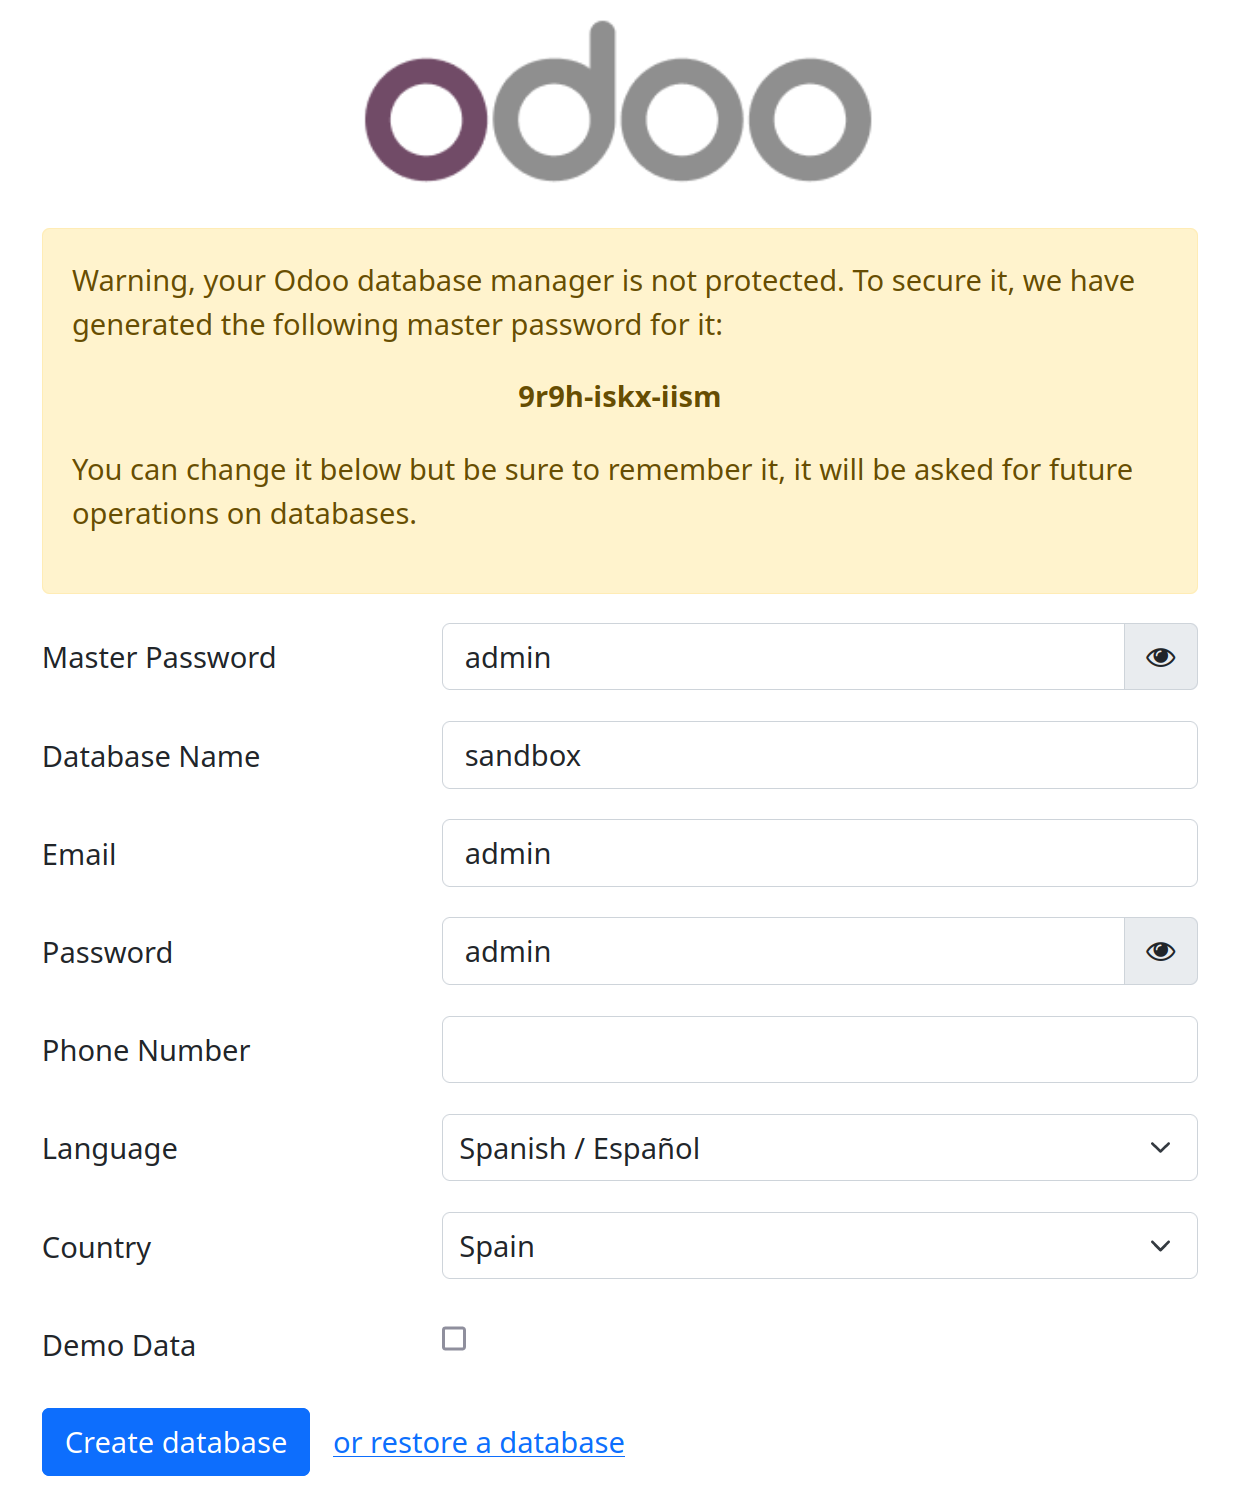
\includegraphics[width=6cm]{instalacion/signup.png}
    \caption{Proceso de registro en Odoo}
    \label{fig:signup}
\end{figure}
\paragraph{}
Por último, cuando se tenga que iniciar sesión, se tendrán que introducir las credenciales previamente definidas.

\subsubsection{Comprobación y creación de sitio web}
\paragraph{}
Con estos pasos se ha conseguido tener instalado Odoo en la máquina de forma local. Para comprobar su correcta instalación, podemos probar el módulo \textit{Blog}. Tras iniciar sesión por primera vez nos redirigirá a la ventana de \textit{Aplicaciones}, en caso contrario se ha de  navegar manualmente. Luego, se ha eliminado el filtro de \textit{Aplicaciones} de la barra de búsqueda y se ha buscado \textit{Blog}.
\paragraph{}
\paragraph{}
Se ha hecho clic en \textit{Activar} dentro de la tarjeta de Blog para instalar automáticamente los módulos relacionados con la web.
\paragraph{}
En este menú, se ha seleccionado la opción de \textit{Vamos a hacerlo}, que permite crear la web de forma sencilla en cuatro pasos. Se ha seleccionado e introducido la información que más se adecua al caso particular y se han personalizado los colores y características de la web. A continuación, se ha creado la web siguiendo la información proporcionada. En este caso, se ha creado una web de venta de coches:
\paragraph{}
\begin{figure}[h]
    \centering
    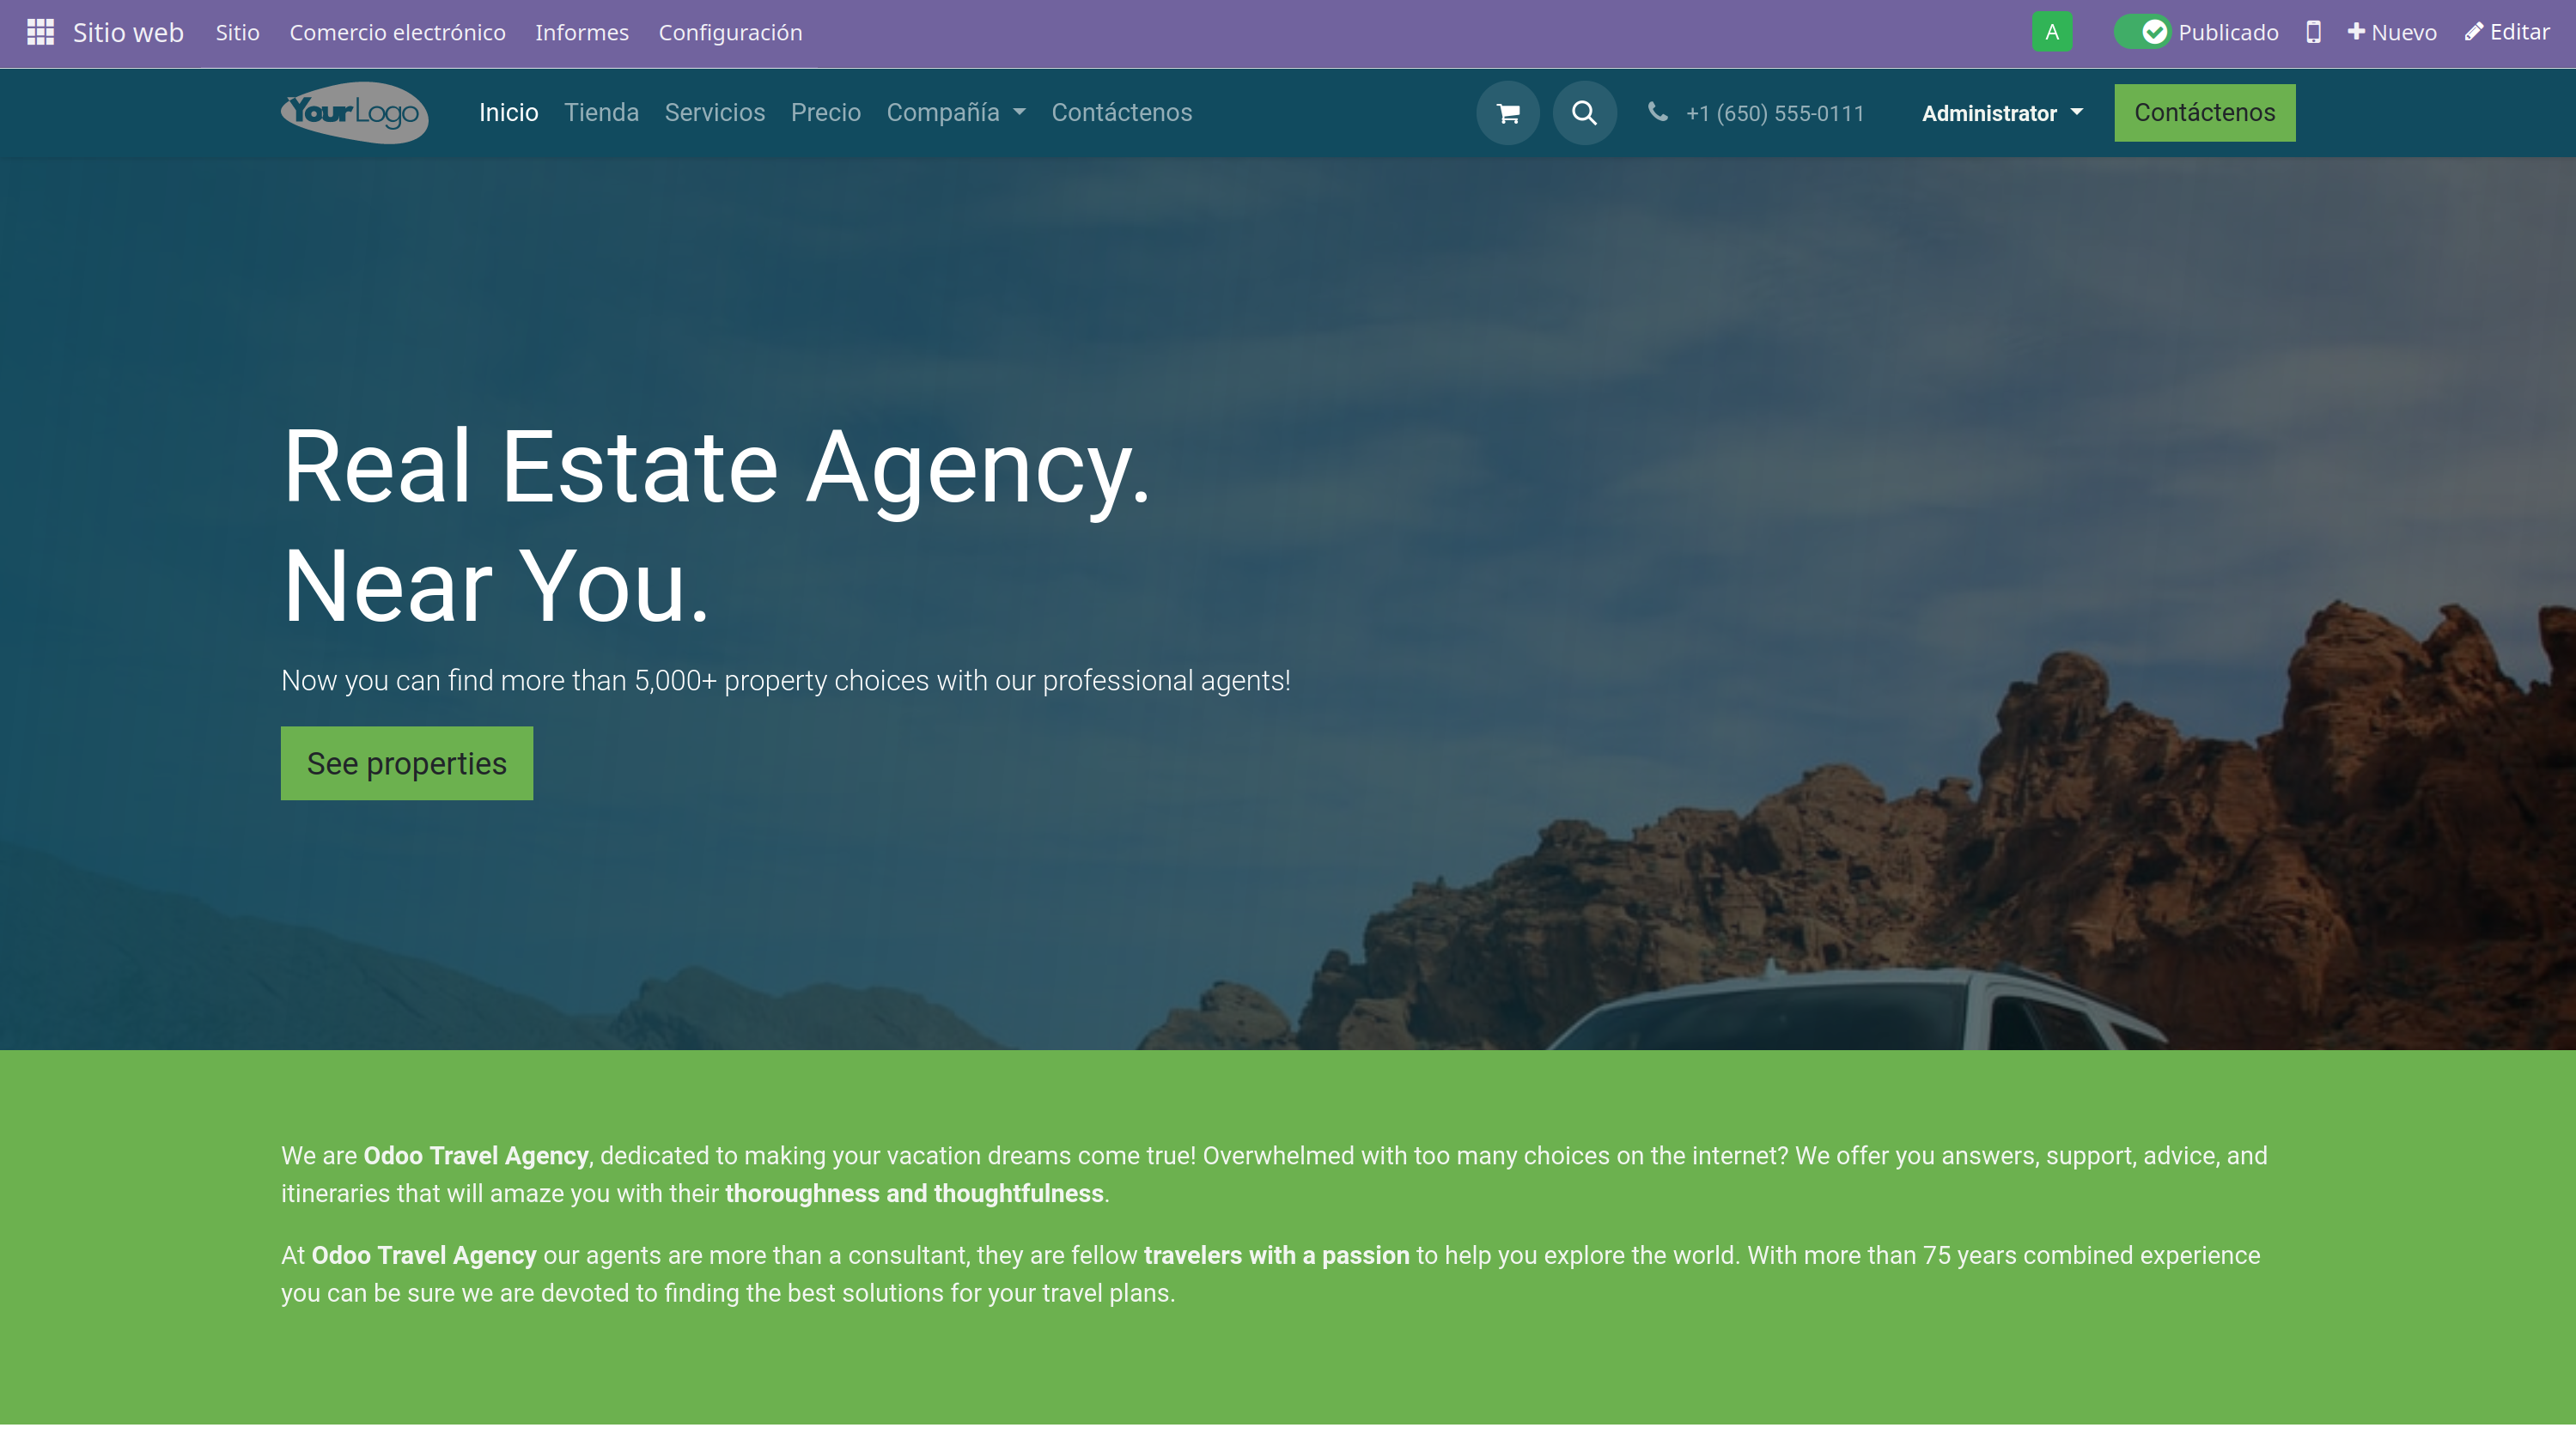
\includegraphics[width=1\linewidth]{instalacion/web.png}
    \caption{Sitio web creado automáticamente}
    \label{fig:web}
\end{figure}
\paragraph{}
Se ha hecho clic en la opción \textit{Nuevo} en la esquina superior derecha y selecciona \textit{Entrada de blog}. Elige un blog existente o crea uno nuevo. Se ha introducido el título de la entrada de blog y pulsa \textit{Guardar}. Se mostrará la entrada de blog creada junto con un menú donde editar esta vista.
\paragraph{}
Si se hace clic en el fondo verde que engloba el título, se puede editar y añadir una imagen al fondo. Además, si se desea añadir una galería de fotos sobre el producto, en este caso un coche, se puede arrastrar la galería de imágenes desde el menú lateral derecho de edición y soltarlo en la parte de la web donde se desea ubicar.
\paragraph{}
Si se hace clic en la galería, se mostrará un menú de edición en el lateral derecho donde se puede editar y personalizar. Para añadir las imágenes que se desean mostrar, haz clic en \textit{Añadir} en la opción de imágenes dentro de la sección \textit{Galería de imágenes} del menú de edición. Luego, haz clic en \textit{Subir archivo} y selecciona las imágenes. Una vez subidas las fotos a Odoo, haz clic en cada imagen de la galería y selecciona la foto a mostrar.
\paragraph{}
Si se quiere dar acceso a la compra del producto mostrado, se añadirá un bloque llamado \textit{Llamamiento a la acción} de la misma manera que se ha hecho la galería de imágenes. Además, se puede editar cualquier texto de la web para adecuar la información a las necesidades.

\begin{figure}[h]
    \centering
    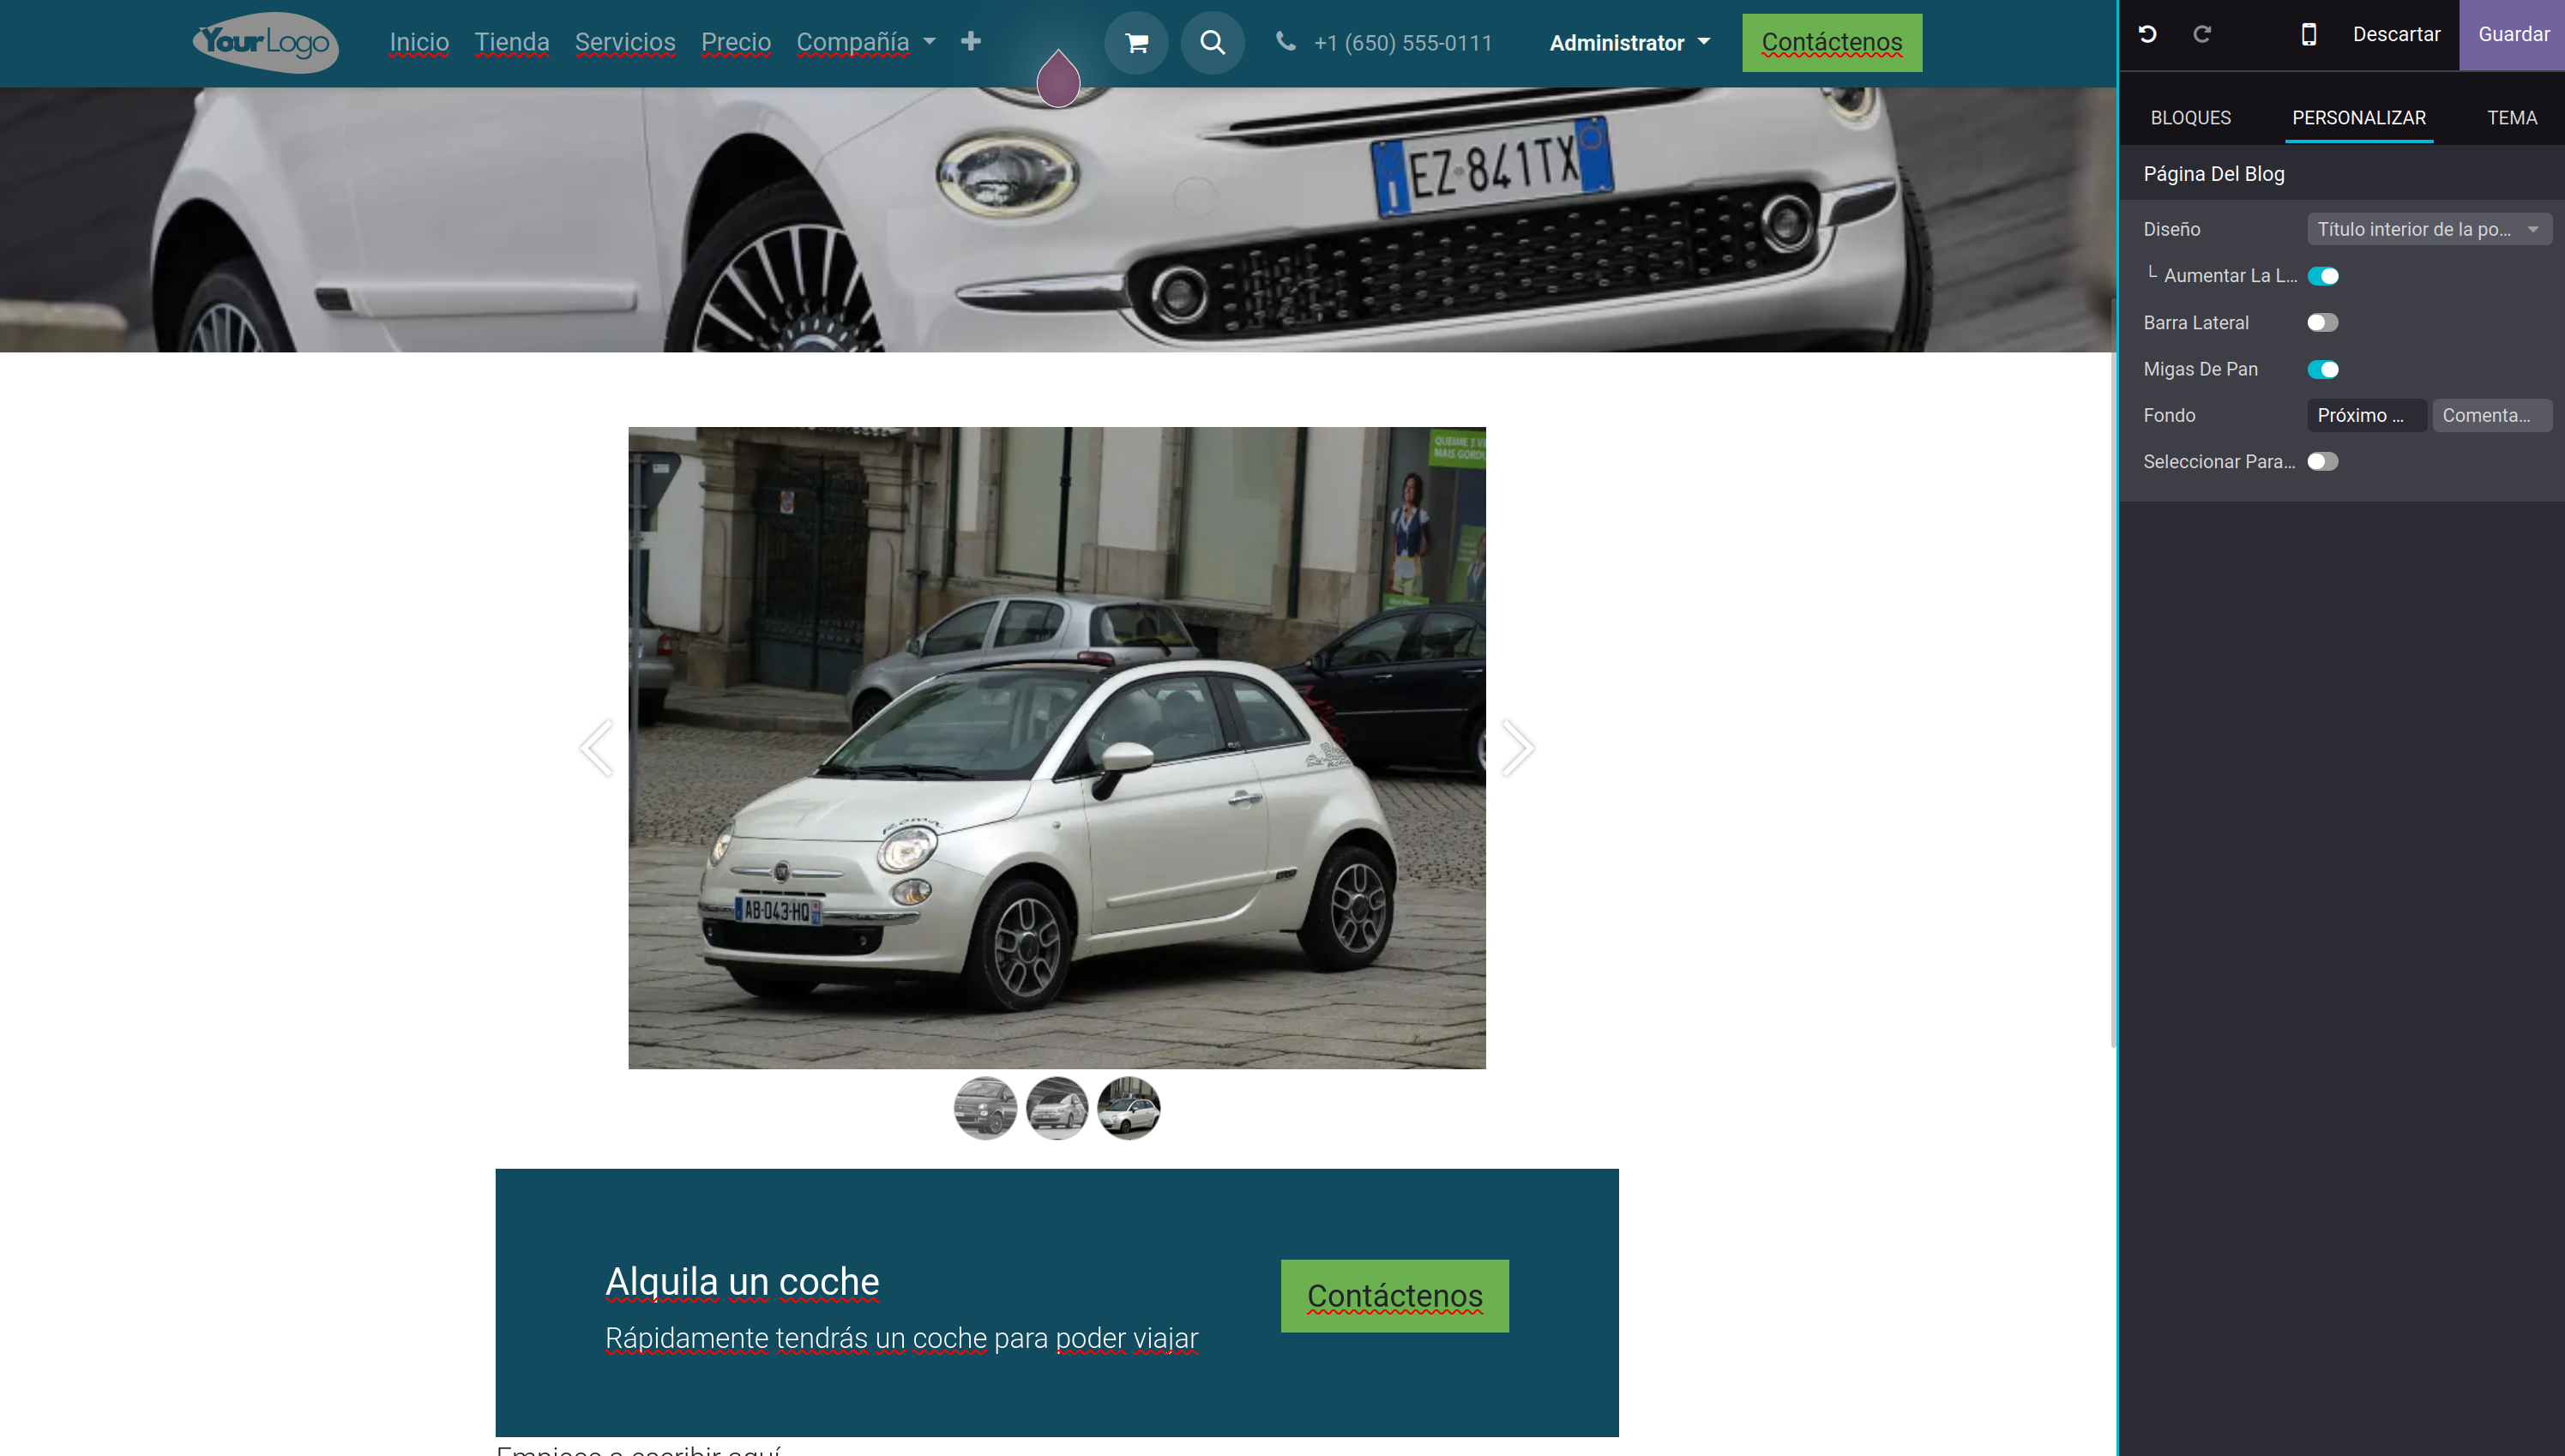
\includegraphics[width=1\linewidth]{instalacion/callToAction.png}
    \caption{Adición de un llamamiento a la acción a la entrada de blog}
    \label{fig:callToAction}
\end{figure}
\paragraph{}
Una vez que la entrada de blog esté personalizado, se ha guardado haciendo clic en el botón \textit{Guardar} en la esquina superior derecha.
\paragraph{}
Para añadir una página nueva al sitio web, se ha añadio una página. Se ha seleccionado la opción \textit{Servicios} del menú lateral izquierdo y se ha elegido la página que más se adecua a tus necesidades. En este caso, se ha creado un sitio con preguntas frecuentes, problemas comunes y sus soluciones, por lo que se ha elegido la segunda opción. Se ha introducido el título de la página, se ha activado la opción \textit{Añadir al menú} y pulsa \textit{Crear}. Edita y personaliza cada texto y foto para que se ajuste a tus necesidades. Nos hemos enfocado en el contenido importante de esta página, que son las preguntas frecuentes y los problemas comunes con sus soluciones. Para ello, se ha utilizado el bloque acordeón que ya existe en la parte inferior de la página. Para añadir nuevos temas, se ha hecho clic en el acordeón y luego en \textit{Añadir artículo} en la opción \textit{Tema} de la sección \textit{Acordeón} del menú lateral derecho. Finalmente, se ha hecho clic en \textit{Guardar} en la esquina superior. Siguiendo estos pasos, conseguimos tener instalado Odoo en nuestras máquinas locales y hemos comprobado su correcto funcionamiento desarrollando un sitio web para nuestra empresa con entradas de blog.

\subsubsection{Instalación en máquina remota}
\paragraph{}
Tener Odoo en nuestra máquina local complica el acceso desde cualquier lugar del mundo, por lo que hemos analizado la viabilidad de instalar Odoo en una máquina remota que nos permita acceder desde el navegador. Hemos investigado distintos servicios de \textit{cloud computing}; \href{https://azure.microsoft.com/en-us/}{Azure}, \href{https://aws.amazon.com}{\textit{Amazon Web Service (AWS)}} y \href{https://railway.app}{\textit{Railway.app}}. Tras analizar sus ventajas y desventajas, hemos decidido utilizar \textit{AWS}. Esta decisión se basó en su facilidad para crear una máquina, la intuición de su interfaz de consola para gestionar las máquinas y su \textit{pricing}, ya que al ser una cuenta nueva, tenemos una máquina gratuita durante un periodo de tiempo limitado; suficiente para realizar este análisis.

\paragraph{}
Lo primero que se debe hacer es crear una cuenta en \textit{AWS}. Después de rellenar nuestros datos y crear la cuenta, iniciamos sesión en la consola de \textit{AWS} y nos abrirá el menú principal como en la figura \ref{aws-home}. Seleccionamos el servicio EC2 para lanzar una instancia. Se nos redirigirá a una página donde debemos configurar la máquina que vamos a usar. En nuestro caso, hemos seleccionado un Ubuntu con la configuración predeterminada propuesta por Amazon.

\begin{figure}[h]
    \centering
    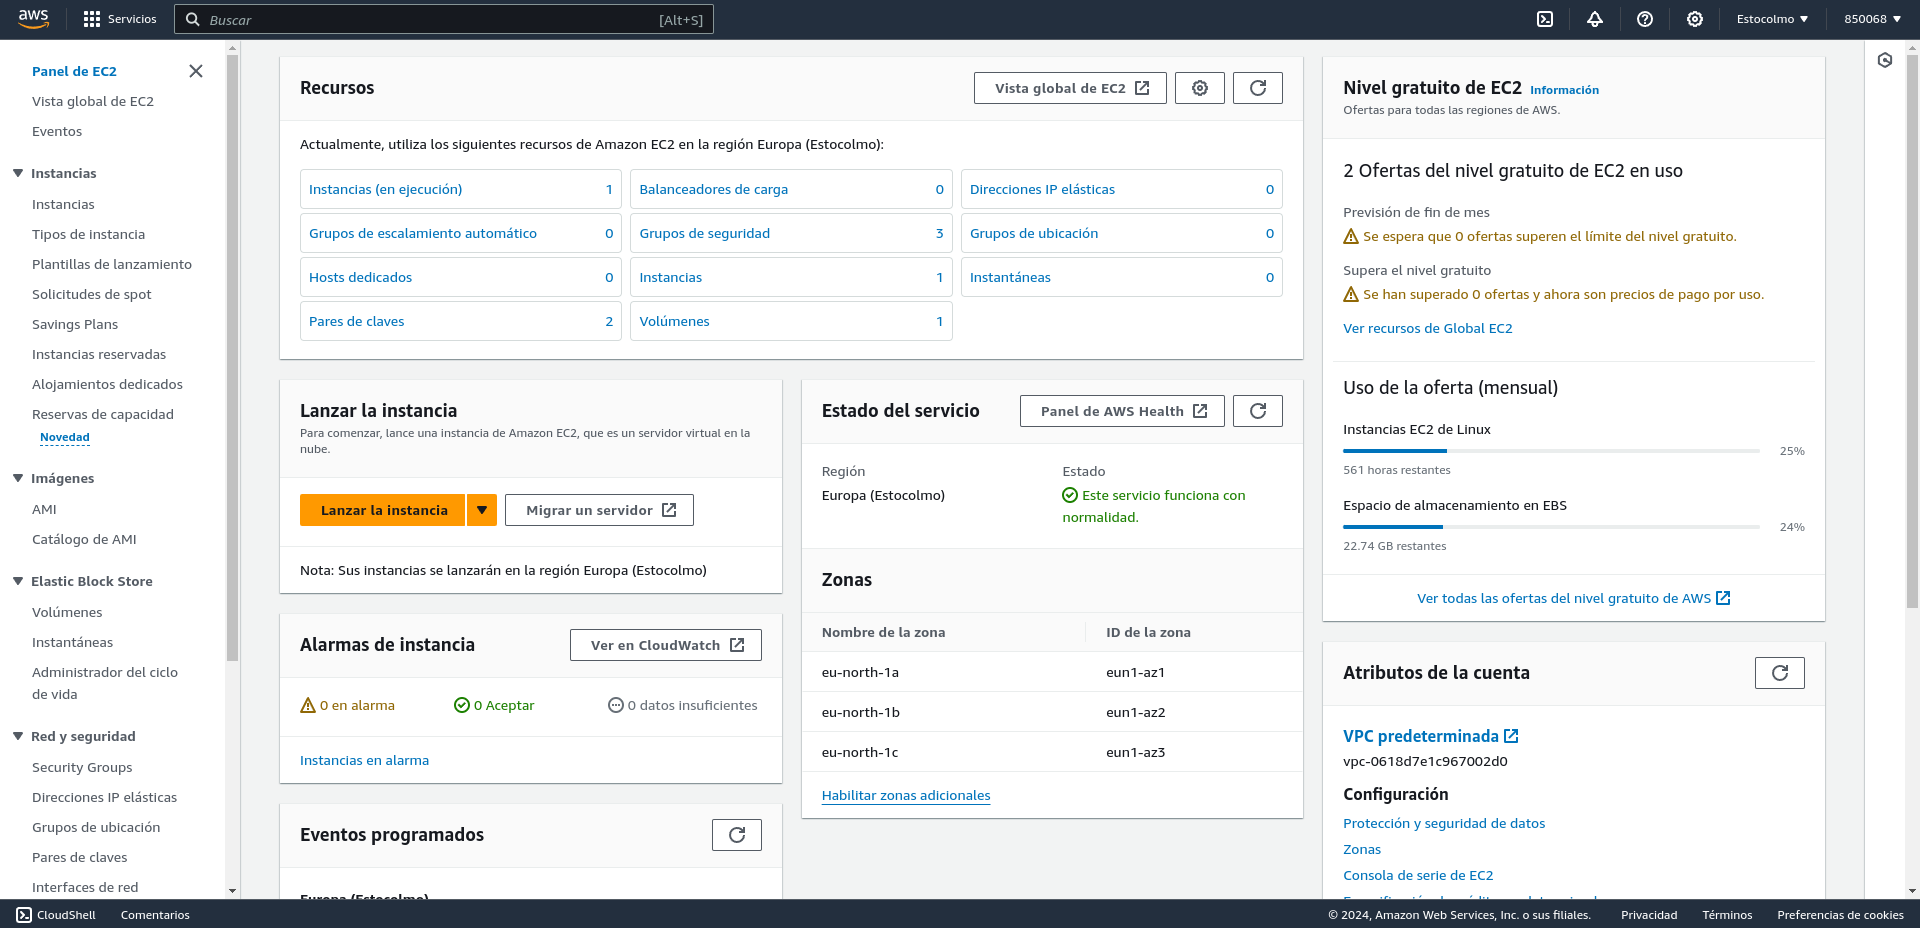
\includegraphics[width=1\linewidth]{instalacion/aws.png}
    \caption{Consola AWS}
    \label{aws-home}
\end{figure}

\paragraph{}
Una vez que se ha creado la instancia, se deben crear un par de claves para acceder a la máquina. Seleccionamos en el menú \textit{Red y seguridad} \textgreater{} \textit{Pares de claves} \textgreater{} \textit{Crear par de claves}. Introducimos el nombre que deseamos y creamos el par de claves. Se descargará la clave recién creada.

\paragraph{}
Por último, debemos configurar las reglas de seguridad para permitir el tráfico HTTPS en el puerto 8069. Para ello, seleccionamos en el panel lateral \textit{Grupos de seguridad} \textgreater{} \textit{Crear grupo de seguridad}. Introducimos el nombre que deseamos y agregamos una regla de entrada: debe ser TCP personalizado con intervalo de puertos de 8069. Guardamos las reglas y ya podremos desplegar el contenedor con Odoo en nuestra máquina EC2.

\paragraph{}
Para realizar la conexión a nuestra máquina, abrimos una terminal e introducimos el siguiente comando en un ordenador MacOS o Linux:

\begin{lstlisting}[frame=single, basicstyle=\small]
ssh -i "ruta/a/tu/clave.pem" usuario@direccion-IP-de-la-instancia
\end{lstlisting}

\paragraph{}
Donde se deben sustituir los campos por los que correspondan. Una vez que se ha realizado la conexión SSH con la máquina, se deben seguir los mismos pasos explicados previamente para lanzar Odoo en la sección de instalación local.

\subsection{Resultados y análisis}
\paragraph{}
Una vez completada la instalación de Odoo tanto en una máquina local como en una máquina remota, se realizaron pruebas de funcionamiento para evaluar la efectividad de ambos métodos.

\subsubsection{Instalación local}
\paragraph{}
La instalación de Odoo localmente permitió verificar que el sistema se ejecuta de manera eficiente y rápida, brindando acceso a todas las funcionalidades del ERP sin mayores problemas. Además, el uso de Docker facilitó la gestión de las dependencias y la configuración, reduciendo el riesgo de errores de compatibilidad.
\paragraph{}
Sin embargo, operar localmente limita el acceso a Odoo a la máquina específica donde está instalado, lo que puede dificultar la colaboración remota o el acceso desde distintos dispositivos y ubicaciones.

\subsubsection{Instalación en máquina remota}
\paragraph{}
La instalación de Odoo en una máquina remota, utilizando los servicios de \textit{AWS}, permitió acceder al sistema desde cualquier lugar con conexión a internet. Esta flexibilidad facilita la colaboración entre diferentes equipos y departamentos, al permitir el acceso simultáneo y remoto a Odoo.
\paragraph{}
Durante las pruebas, se comprobó que la instalación remota ofrece un rendimiento similar al local, con la ventaja adicional de la escalabilidad que ofrece la infraestructura de \textit{AWS}. Esta opción es especialmente útil para nuestra empresa, dadas las necesidades de acceso distribuido y el posible alto volumen de usuarios.

\subsubsection{Comparación}
\paragraph{}
En resumen, aunque la instalación local ofrece mayor control sobre el sistema, la instalación remota brinda flexibilidad y escalabilidad para el acceso desde cualquier ubicación. Dependiendo de las necesidades específicas de la empresa, ambas opciones pueden ser adecuadas, aunque se recomienda la instalación remota debido a la necesidad de acceso desde múltiples ubicaciones y una infraestructura escalable.

\subsection{Conclusiones}
\paragraph{}
En base a los resultados obtenidos durante la instalación y prueba de Odoo, se pueden extraer las siguientes conclusiones:

\begin{itemize}
    \item La instalación de Odoo localmente es adecuada para entornos de desarrollo o pruebas, donde se requiere acceso rápido y control directo sobre el sistema.
    \item La instalación remota, utilizando servicios de \textit{cloud computing} como \textit{AWS}, ofrece una solución escalable y flexible que permite el acceso desde cualquier ubicación con conexión a internet.
    \item La instalación remota es especialmente recomendable para entornos empresariales que requieran acceso distribuido y colaboración entre diferentes equipos y departamentos.
    \item Se recomienda continuar utilizando la instalación remota para aprovechar la escalabilidad y flexibilidad que ofrece la infraestructura en la nube.
\end{itemize}
\paragraph{}
En general, la instalación de Odoo, tanto local como remota, demuestra ser una solución efectiva para la gestión empresarial, permitiendo optimizar y agilizar los procesos internos de la empresa.
